\documentclass[a4paper,12pt]{article} % тип документа

% Поля страниц
\usepackage[left=2.5cm,right=2.5cm, top=2cm,bottom=2cm,bindingoffset=0cm]{geometry}
    
%Пакет дял таблиц   
\usepackage{multirow} 
    
%Отступ после заголовка    
\usepackage{indentfirst}


% Рисунки
\usepackage{subcaption,floatrow,graphicx,calc}
\usepackage{wrapfig}

% Создаёем новый разделитель
\DeclareFloatSeparators{mysep}{\hspace{1cm}}

% Ссылки?
\usepackage{hyperref}
\usepackage[rgb]{xcolor}
\hypersetup{				% Гиперссылки
    colorlinks=true,       	% false: ссылки в рамках
	urlcolor=blue          % на URL
}


%  Русский язык
\usepackage[T2A]{fontenc}			% кодировка
\usepackage[utf8]{inputenc}			% кодировка исходного текста
\usepackage[english,russian]{babel}	% локализация и переносы


% Математика
\usepackage{amsmath,amsfonts,amssymb,amsthm,mathtools, mathrsfs, wasysym}


\begin{document}
\begin{center}
	\footnotesize{ФЕДЕРАЛЬНОЕ ГОСУДАРСТВЕННОЕ АВТОНОМНОЕ ОБРАЗОВАТЕЛЬНОЕ 			УЧРЕЖДЕНИЕ ВЫСШЕГО ОБРАЗОВАНИЯ}\\
	\footnotesize{МОСКОВСКИЙ ФИЗИКО-ТЕХНИЧЕСКИЙ ИНСТИТУТ\\(НАЦИОНАЛЬНЫЙ 			ИССЛЕДОВАТЕЛЬСКИЙ УНИВЕРСИТЕТ)}\\
	\footnotesize{ФАКУЛЬТЕТ ОБЩЕЙ И ПРИКЛАДНОЙ ФИЗИКИ\\}
	\hfill \break
	\hfill\break
	\hfill\break
	\hfill \break
	\hfill \break
	\hfill \break
	\hfill \break
	\hfill \break
	\hfill \break
	\hfill \break
	\hfill \break
	\hfill \break
	\hfill \break
	\hfill \break
	\large{Лабораторная работа № 5.4.1 \\\textbf{Определение энергии $\alpha$-частиц\\по величине их пробега в воздухе}}\\
	\hfill \break
	\hfill \break
	\hfill \break
	\begin{flushright}
		Серебренников Даниил\\
		Группа Б02-826м
	\end{flushright}
	\hfill \break
	\hfill \break
	\hfill \break
	\hfill \break
	\hfill \break
	\hfill \break
	\hfill \break
	\hfill \break
	\hfill \break
	\hfill \break
	\hfill \break
\end{center}
\begin{center}
	Долгопрудный, 2020 г.
\end{center}
\thispagestyle{empty}
\newpage
	\textbf{Цель работы:} измерить пробег $\alpha$-частиц в воздухе двумя способами: с помощью торцевого счетчика Гейгера и синтиляционного счетчика, -- по полученным данным определить энергию частиц.

\section{Теоретическая часть}
	При $\alpha$-распаде исходное родительское ядро испускает ядро гелия и превращается в дочернее ядро, число протонов и число протонов уменьшается на две единицы. Функциональная свзяь между энергией $\alpha$-частицы $E$ и периодом полураспада радиоактивного ядра $T_{1/2}$ хорошо описывается формулой
	\begin{equation*}
		 \lg T_{1/2} = \frac{a}{\sqrt{E}} + b.
	\end{equation*}
	Экспоненциальный характер этого процесса возникает вследствие экспоненциального затухания волновой функции в области под барьером, где потенциальная энергия больше энергии частицы.
	
	Для описания связи между энергией $\alpha$-частицы и ее пробегом пользуются эмпирическими соотношениями. В диапазоне энергий $\alpha$-частиц от 4 до 9 МэВ эта связь хорошо описывается выражением
	\begin{equation*}
		\label{eq:R(E)}
		\tag{$\star$}
		R = 0,32E^{3/2}
	\end{equation*}
	

\section{Экспериментальная установка}
	В данной работе пробег $\alpha$-частиц в воздухе определяется треями способами:
	\begin{enumerate}
		\item
			С помощью счетчика Гейгера -- рис.~\ref{pic1};
		\item
			C помощью сцинтилляционного счетчика -- рис.~\ref{pic2};
		\item
			C помощью ионизационной камеры -- рис.~\ref{pic3}.
	\end{enumerate} 
	
	\thisfloatsetup{floatrowsep=mysep}	
	\begin{figure}[h!]
		\ffigbox{
			\begin{subfloatrow}[3]
				\ffigbox[\FBwidth]{\caption{}}%
				{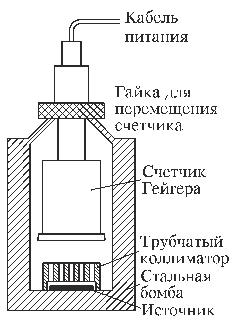
\includegraphics[scale=1]{ustanovka1.pdf}{\label{pic1}}}
				\ffigbox[\FBwidth]{\caption{}}%
				{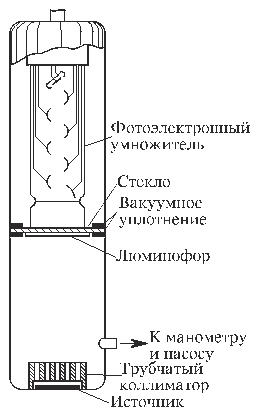
\includegraphics[scale=0.8]{ustanovka2.pdf}{\label{pic2}}}
				\ffigbox[\FBwidth]{\caption{}}%
				{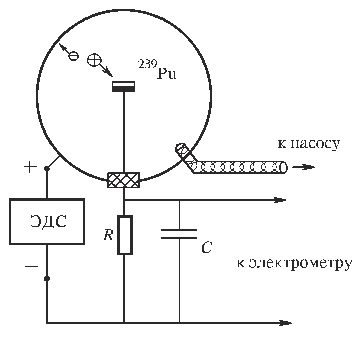
\includegraphics[scale=1]{ustanovka3.pdf}{\label{pic3}}}          
			\end{subfloatrow}
		}
		{\caption{Экспериментальные установки.}}
	\end{figure}
	
	В качестве источника $\alpha$-частиц используется ${239}$Pu с периодом полураспада $T_{1/2} = 2,44 \cdot 10^4$ лет. Альфа-частицы, испускаемые ${239}$Pu состоят их трех моноэнергетических групп, различие между которыми лежит в пределах 50 кэВ. При той точности, которая достигается в наших опытах, их можно считать совпадающими по энергии, равной 5,15 МэВ.
	
	
	\newpage
	\section{Экспериментальные данные}
		\floatsetup[table]{capposition=top}	
		\begin{table}[H]
			\caption{Ионизационная камера.}
			\label{table:exp3}
			\begin{tabular}{|c|c|c|c|}
				\hline
				$P$, торр & $\sigma_P$, торр    & $I$, пА & $\sigma_I$, пА \\ \hline
				18        & \multirow{35}{*}{3} & 16      & 1              \\ \cline{1-1} \cline{3-4} 
				38        &                     & 43      & 1              \\ \cline{1-1} \cline{3-4} 
				58        &                     & 71      & 1              \\ \cline{1-1} \cline{3-4} 
				78        &                     & 101     & 1              \\ \cline{1-1} \cline{3-4} 
				98        &                     & 130     & 1              \\ \cline{1-1} \cline{3-4} 
				118       &                     & 160     & 1              \\ \cline{1-1} \cline{3-4} 
				138       &                     & 193     & 1              \\ \cline{1-1} \cline{3-4} 
				158       &                     & 221     & 1              \\ \cline{1-1} \cline{3-4} 
				208       &                     & 304     & 5              \\ \cline{1-1} \cline{3-4} 
				258       &                     & 388     & 5              \\ \cline{1-1} \cline{3-4} 
				308       &                     & 470     & 5              \\ \cline{1-1} \cline{3-4} 
				368       &                     & 576     & 5              \\ \cline{1-1} \cline{3-4} 
				468       &                     & 765     & 5              \\ \cline{1-1} \cline{3-4} 
				478       &                     & 795     & 5              \\ \cline{1-1} \cline{3-4} 
				498       &                     & 827     & 5              \\ \cline{1-1} \cline{3-4} 
				518       &                     & 875     & 5              \\ \cline{1-1} \cline{3-4} 
				538       &                     & 911     & 5              \\ \cline{1-1} \cline{3-4} 
				548       &                     & 927     & 5              \\ \cline{1-1} \cline{3-4} 
				558       &                     & 940     & 5              \\ \cline{1-1} \cline{3-4} 
				578       &                     & 960     & 5              \\ \cline{1-1} \cline{3-4} 
				598       &                     & 966     & 5              \\ \cline{1-1} \cline{3-4} 
				608       &                     & 971     & 5              \\ \cline{1-1} \cline{3-4} 
				618       &                     & 970     & 5              \\ \cline{1-1} \cline{3-4} 
				628       &                     & 966     & 5              \\ \cline{1-1} \cline{3-4} 
				638       &                     & 964     & 5              \\ \cline{1-1} \cline{3-4} 
				658       &                     & 962     & 10             \\ \cline{1-1} \cline{3-4} 
				668       &                     & 963     & 10             \\ \cline{1-1} \cline{3-4} 
				678       &                     & 957     & 10             \\ \cline{1-1} \cline{3-4} 
				688       &                     & 960     & 10             \\ \cline{1-1} \cline{3-4} 
				708       &                     & 953     & 10             \\ \cline{1-1} \cline{3-4} 
				718       &                     & 952     & 10             \\ \cline{1-1} \cline{3-4} 
				728       &                     & 945     & 10             \\ \cline{1-1} \cline{3-4} 
				738       &                     & 944     & 10             \\ \cline{1-1} \cline{3-4} 
				748       &                     & 940     & 10             \\ \cline{1-1} \cline{3-4} 
				758       &                     & 937     & 10             \\ \hline
			\end{tabular}
		\end{table}
	
		\floatsetup[table]{capposition=top}	
		\begin{table}[H]
			\caption{Счетчик Гейгера.}
			\label{table:exp1}
			\begin{tabular}{|c|c|c|c|c|c|}
				\hline
				$t$, с & $N_0$ & $x$, мм & $\sigma_x$, мм        & $N$  & $\sigma_N$ \\ \hline
				102    & 15    & 40,0    & \multirow{20}{*}{0,5} & 14,7 & 0,7        \\ \cline{1-3} \cline{5-6} 
				202    & 25    & 35,0    &                       & 12,4 & 0,3        \\ \cline{1-3} \cline{5-6} 
				141    & 15    & 30,0    &                       & 10,6 & 0,4        \\ \cline{1-3} \cline{5-6} 
				115    & 24    & 28,0    &                       & 20,9 & 0,9        \\ \cline{1-3} \cline{5-6} 
				124    & 27    & 26,0    &                       & 21,8 & 0,9        \\ \cline{1-3} \cline{5-6} 
				1345   & 25    & 24,0    &                       & 1,86 & 0,01       \\ \cline{1-3} \cline{5-6} 
				210    & 45    & 23,0    &                       & 21,4 & 0,5        \\ \cline{1-3} \cline{5-6} 
				200    & 46    & 22,0    &                       & 23,0 & 0,6        \\ \cline{1-3} \cline{5-6} 
				250    & 73    & 21,0    &                       & 29,2 & 0,6        \\ \cline{1-3} \cline{5-6} 
				218    & 76    & 20,0    &                       & 34,9 & 0,8        \\ \cline{1-3} \cline{5-6} 
				111    & 238   & 19,0    &                       & 214  & 10         \\ \cline{1-3} \cline{5-6} 
				136    & 1000  & 18,0    &                       & 735  & 30         \\ \cline{1-3} \cline{5-6} 
				115    & 1583  & 17,0    &                       & 1380 & 60         \\ \cline{1-3} \cline{5-6} 
				120    & 1800  & 16,0    &                       & 1500 & 60         \\ \cline{1-3} \cline{5-6} 
				109    & 1600  & 15,0    &                       & 1470 & 70         \\ \cline{1-3} \cline{5-6} 
				105    & 1561  & 14,0    &                       & 1490 & 70         \\ \cline{1-3} \cline{5-6} 
				103    & 1536  & 13,0    &                       & 1490 & 70         \\ \cline{1-3} \cline{5-6} 
				110    & 1564  & 12,0    &                       & 1420 & 60         \\ \cline{1-3} \cline{5-6} 
				113    & 1560  & 11,0    &                       & 1380 & 60         \\ \cline{1-3} \cline{5-6} 
				103    & 1484  & 10,0    &                       & 1440 & 70         \\ \hline
			\end{tabular}
		\end{table}
		
		\floatsetup[table]{capposition=top}	
		\begin{table}[H]
			\caption{Сцинтилляционный счетчик.}
			\label{table:exp2}
			\begin{tabular}{|c|c|c|c|c|c|}
				\hline
				$t$, с & $N_0$ & $P$, торр & $\sigma_P$, торр    & $N$, $10^3$ & $\sigma_N$, $10^3$ \\ \hline
				10     & 3603  & 18        & \multirow{22}{*}{3} & 36          & 2                  \\ \cline{1-3} \cline{5-6} 
				10     & 3435  & 38        &                     & 34          & 2                  \\ \cline{1-3} \cline{5-6} 
				10     & 3233  & 58        &                     & 32          & 2                  \\ \cline{1-3} \cline{5-6} 
				10     & 3089  & 78        &                     & 31          & 2                  \\ \cline{1-3} \cline{5-6} 
				10     & 2923  & 98        &                     & 29          & 1                  \\ \cline{1-3} \cline{5-6} 
				10     & 2744  & 108       &                     & 27          & 1                  \\ \cline{1-3} \cline{5-6} 
				10     & 2646  & 118       &                     & 26          & 1                  \\ \cline{1-3} \cline{5-6} 
				10     & 2347  & 138       &                     & 23          & 1                  \\ \cline{1-3} \cline{5-6} 
				10     & 2036  & 158       &                     & 20          & 1                  \\ \cline{1-3} \cline{5-6} 
				10     & 1992  & 166       &                     & 20          & 1                  \\ \cline{1-3} \cline{5-6} 
				10     & 1830  & 176       &                     & 18,3        & 0,9                \\ \cline{1-3} \cline{5-6} 
				10     & 1666  & 186       &                     & 16,7        & 0,8                \\ \cline{1-3} \cline{5-6} 
				10     & 1431  & 196       &                     & 14,3        & 0,7                \\ \cline{1-3} \cline{5-6} 
				10     & 1260  & 208       &                     & 12,6        & 0,6                \\ \cline{1-3} \cline{5-6} 
				10     & 1001  & 216       &                     & 10,0        & 0,5                \\ \cline{1-3} \cline{5-6} 
				10     & 820   & 226       &                     & 8,2         & 0,4                \\ \cline{1-3} \cline{5-6} 
				10     & 635   & 236       &                     & 6,4         & 0,3                \\ \cline{1-3} \cline{5-6} 
				10     & 474   & 246       &                     & 4,7         & 0,2                \\ \cline{1-3} \cline{5-6} 
				10     & 324   & 258       &                     & 3,2         & 0,2                \\ \cline{1-3} \cline{5-6} 
				10     & 90    & 276       &                     & 0,90        & 0,05               \\ \cline{1-3} \cline{5-6} 
				100    & 51    & 308       &                     & 0,0510      & 0,0003             \\ \cline{1-3} \cline{5-6} 
				100    & 11    & 358       &                     & 0,01100     & 0,00006            \\ \hline
			\end{tabular}
		\end{table}
		
		
	
		
	
	\newpage
	\section{Обработка результатов}
		\subsection{Исследование пробега $\alpha$-ч. счетчика Гейгера}	
		Представим результаты измерений (табл.~\ref{table:exp1}) зависимости $N=N(x)$ в виде графика -- рис.~\ref{fig:N(x)}. 
		
		\begin{figure}[h!]
			\begin{floatrow}
				\ffigbox[\FBwidth]{\caption{$N=N(x)$.}\label{fig:N(x)}}%
				{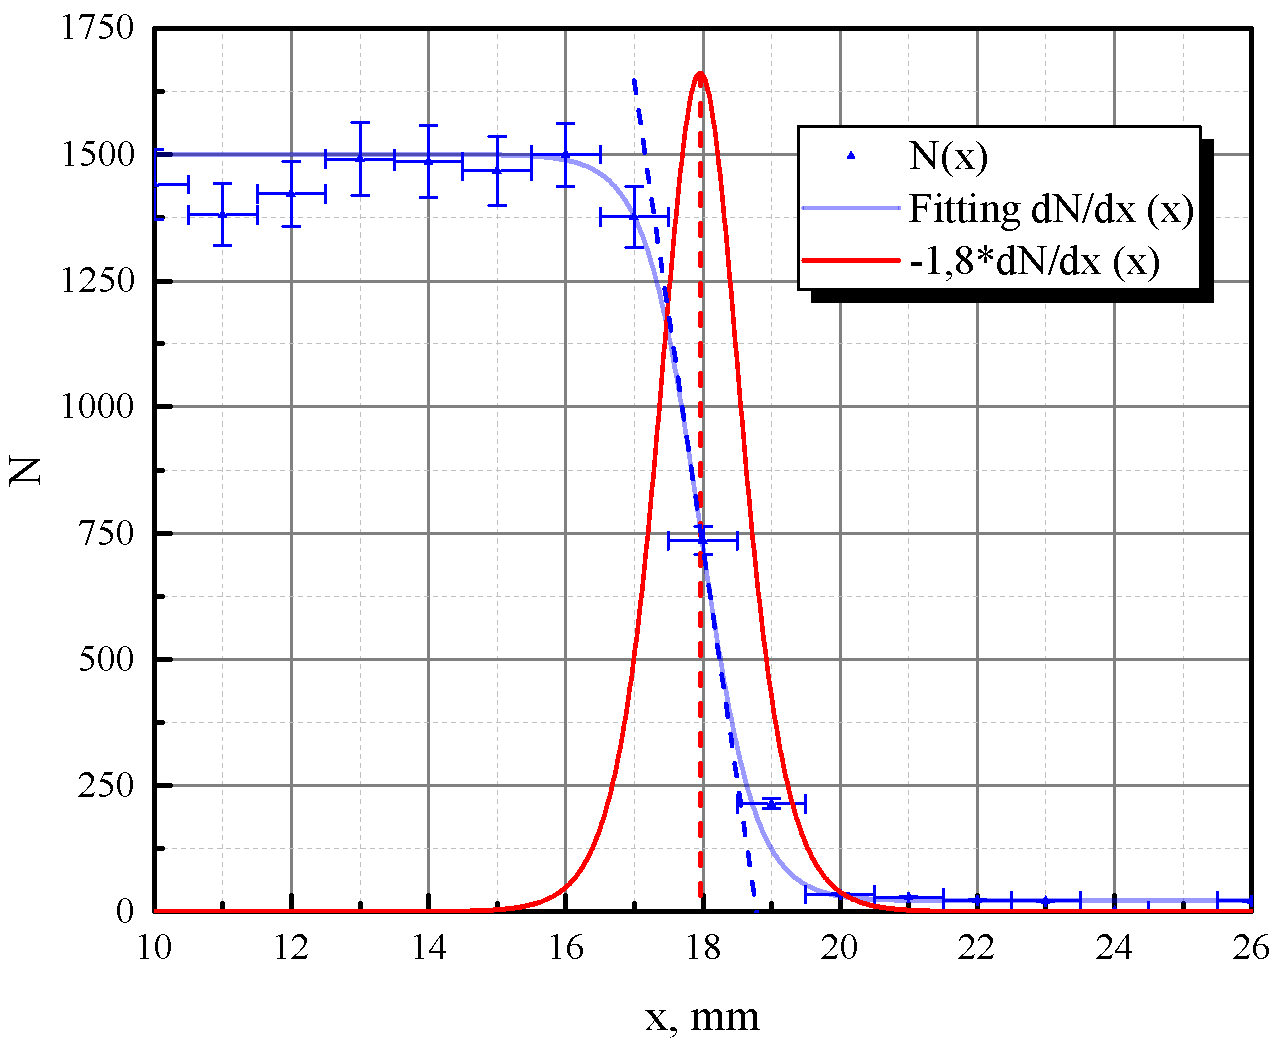
\includegraphics[scale=0.5]{graph1.pdf}}    
			\end{floatrow}
		\end{figure}
	
		Найдем кривую, приближающую экспериментальные точки, в следующем виде:
		\begin{equation*}
			N (x) = \frac{A_1-A_2}{1+e^{(x-x_0)/dx}} + A_2.
		\end{equation*}
	
		\floatsetup[table]{capposition=top}	
		\begin{table}[H]
			\caption{Параметры аппроксимации.}
			\label{tab:pfrfmetry1}
			\begin{tabular}{|c|c|c|c|c|}
				\hline
				$A_1$ & $A_2$ & $x_0$, мм & $dx$, мм & $R^2$ \\ \hline
				1500  & 23    & 18        & 0,4      & ?     \\ \hline
			\end{tabular}
		\end{table}
	
		Средний $R_\text{ср}$ и экстраполированный $R_\text{экстр}$ пробеги определяются следующими уравнениями:
		\begin{equation*}
			\begin{cases}
				N^{\prime \prime} (R_\text{ср}) = 0, \\
				R_\text{экстр} = R_\text{ср} + \left|N(R_\text{ср})/N^\prime(R_\text{ср})\right|.
			\end{cases}
		\end{equation*}
	
		Энергию можно найти из формулы (\ref{eq:R(E)}): $E = \left(R/0,32\right)^{2/3}$.
	
			\begin{table}[h!]
			\begin{floatrow}
				\ttabbox[\FBwidth]{\caption{$R$.}\label{tab:R1}}%
				{\begin{tabular}{|c|c|}
						\hline
						$R_\text{ср}$, см & $R_\text{экстр}$, см \\ \hline
						$1,80 \pm 0,05 $   & $1,9 \pm 0,1$       \\ \hline
				\end{tabular}}
				\ttabbox[\FBwidth]{\caption{$E$.}\label{tab:E1}}%
				{\begin{tabular}{|c|c|}
						\hline
						$E(R_\text{ср})$, МэВ & $E(R_\text{экстр})$, МэВ \\ \hline
						$3,16 \pm 0,06 $     & $3,28 \pm 0,12 $        \\ \hline
				\end{tabular}}        
			\end{floatrow}
		\end{table}
	
	
		\newpage
		\subsection{Исследование пробега $\alpha$-ч. с помощью сцинтилляционного счетчика}	
		Представим результаты измерений (табл.~\ref{table:exp2}) зависимости $N=N(P)$ в виде графика -- рис.~\ref{fig:N(P)}. 
		
		\begin{figure}[h!]
			\begin{floatrow}
				\ffigbox[\FBwidth]{\caption{$N=N(P)$.}\label{fig:N(P)}}%
				{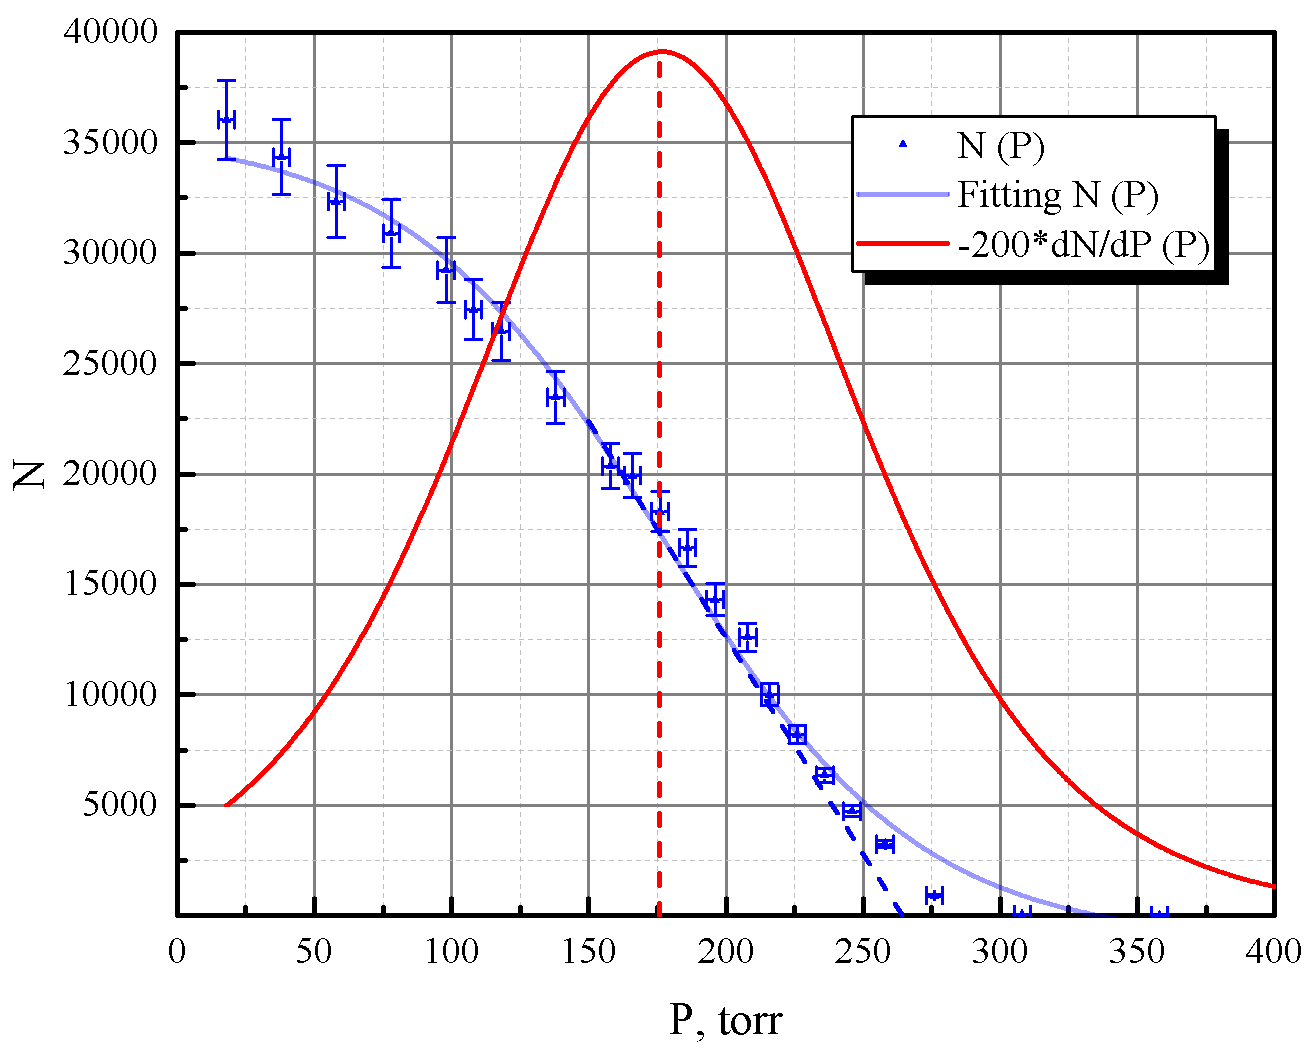
\includegraphics[scale=0.5]{graph2.pdf}}    
			\end{floatrow}
		\end{figure}
		
		Найдем кривую, приближающую экспериментальные точки, в следующем виде:
		\begin{equation*}
			N (P) = \frac{B_1-B_2}{1+e^{(P-P_0)/dP}} + B_2.
		\end{equation*}
		
		\floatsetup[table]{capposition=top}	
		\begin{table}[H]
			\caption{Параметры аппроксимации.}
			\label{tab:parametry2}
			\begin{tabular}{|c|c|c|c|c|}
				\hline
				$B_1$ & $B_2$ & $P_0$, торр & $dP$, торр & $R^2$ \\ \hline
				$35500 \pm 900$  & $-1200 \pm 600$    & $177\pm 4$        & $47\pm 3$      & 0,99     \\ \hline
			\end{tabular}
		\end{table}
		
		Давления $P_\text{ср}$ и $P_\text{экстр}$, которые соответсвуют среднему $R_\text{ср}$ и экстраполированному $R_\text{экстр}$ пробегам, очевидно, определяются следующей системой уравнений:
		\begin{equation*}
			\begin{cases}
				N^{\prime \prime} (P_\text{ср}) = 0, \\
				P_\text{экстр} = P_\text{ср} + \left|N(P_\text{ср})/N^\prime(P_\text{ср})\right|.
			\end{cases}
		\end{equation*}
	
		\floatsetup[table]{capposition=top}	
		\begin{table}[H]
			\caption{P.}
			\label{tab:P}
			\begin{tabular}{|c|c|}
				\hline
				$P_\text{ср}$, торр & $P_\text{экстр}$, торр \\ \hline
				$177 \pm 4 $   & $264 \pm 8$       \\ \hline
			\end{tabular}
		\end{table}
	
		\newpage
		Так как $\alpha$-частицы не могут достигнуть люминофора при обычном давлении, то свободный пробег будет равен расстоянию между препаратом и люминофором -- 9 см. Следовательно, мы можем пересчитать средний и экстраполированные свободные пробеги частиц к давлению 760 торр и температуре 15$^\circ$:
		\begin{equation*}
			R = \frac{288 \ \text{К}}{T}\frac{P}{760 \ \text{торр}}\, 9 \ \text{см}.
		\end{equation*}
		
		\begin{table}[h!]
			\begin{floatrow}
				\ttabbox[\FBwidth]{\caption{$R$.}\label{tab:R2}}%
				{\begin{tabular}{|c|c|}
						\hline
						$R_\text{ср}$, см & $R_\text{экстр}$, см \\ \hline
						$2,03 \pm 0,05 $   & $3,02 \pm 0,09$       \\ \hline
				\end{tabular}}
				\ttabbox[\FBwidth]{\caption{$E$.}\label{tab:E2}}%
				{\begin{tabular}{|c|c|}
						\hline
						$E(R_\text{ср})$, МэВ & $E(R_\text{экстр})$, МэВ \\ \hline
						$3,43 \pm 0,06 $     & $4,47 \pm 0,09 $        \\ \hline
				\end{tabular}}        
			\end{floatrow}
		\end{table}
	
		\subsection{Определение пробега $\alpha$-ч. с помощью ионизационной камеры}
			Представим результаты измерений (табл.~\ref{table:exp3}) зависимости $I=I(P)$ в виде графика -- рис.~\ref{fig:I(P)}. 
		
		\begin{figure}[h!]
			\begin{floatrow}
				\ffigbox[\FBwidth]{\caption{$I=I(P)$.}\label{fig:I(P)}}%
				{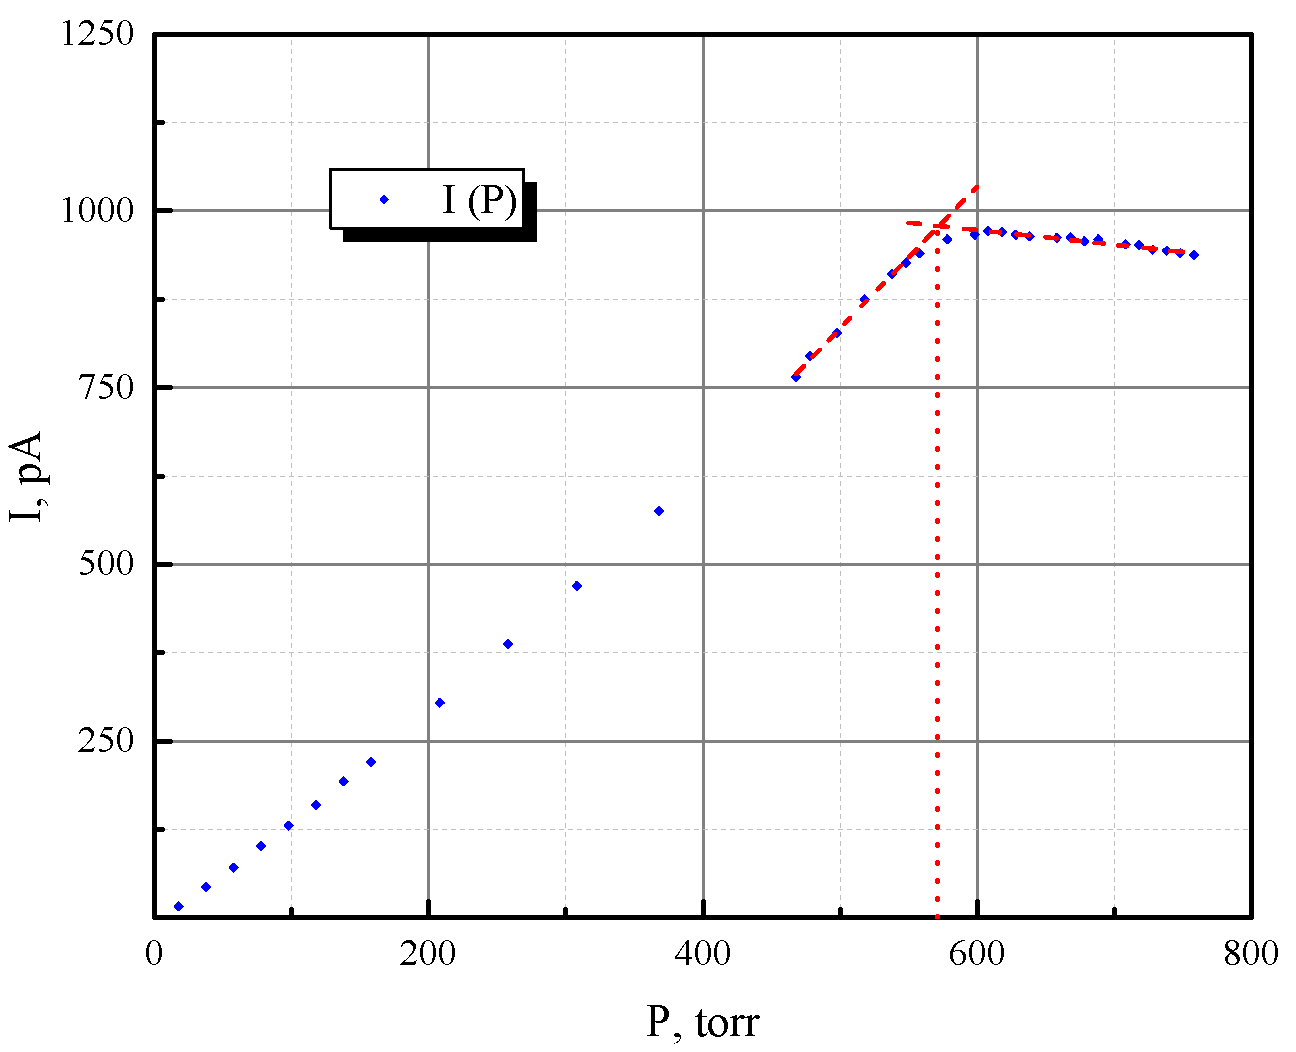
\includegraphics[scale=0.5]{graph3.pdf}}    
			\end{floatrow}
		\end{figure}
		
		По графику определим: $P_\text{экстр} = (570 \pm 10)$ торр. Аналогично предыдущему пункту найдём экстраполированный пробег $R_\text{экстр}$ и соответствующую энергию.
		\begin{equation*}
			R = \frac{288 \ \text{К}}{T}\frac{P}{760 \ \text{торр}}\, \frac{10 - 0.5}{2} \ \text{см},
		\end{equation*}
		где 0.5 см и 10 см -- диаметры первого и второго электродов соответственно.
		\begin{table}[h!]
			\begin{floatrow}
				\ttabbox[\FBwidth]{\caption{$R$.}\label{tab:R3}}%
				{\begin{tabular}{|c|}
						\hline
						$R_\text{экстр}$, см $\ \ \ $ \\ \hline
						$3,44 \pm 0,07$         \\ \hline
				\end{tabular}}
				\ttabbox[\FBwidth]{\caption{$E$.}\label{tab:E3}}%
				{\begin{tabular}{|c|}
						\hline
						$E(R_\text{экстр})$, МэВ \\ \hline
						$4,87 \pm 0,07 $            \\ \hline
				\end{tabular}}        
			\end{floatrow}
		\end{table}
\newpage
\section{Обсуждение результатов и выводы}
	В настоящей лабораторной работе тремя различными способами был измерен свободный пробег в воздухе $\alpha$-частиц  с энергией 5,15 МэВ. В качестве источника радиоактивных частиц был использован $^{239}$Pu.
	
	Результаты вычислений энергий для экстраполированных и средних пробегов (таблицы \ref{tab:E1}, \ref{tab:E2}, \ref{tab:E3}) по эмпирической формуле~(\ref{eq:R(E)}) привели к заниженным значениям. Это обусловлено следующим набором причин:
	\begin{enumerate}
		\item
			Пучки частиц обладают конечными размерами, что приводит к угловой расходимости.
		\item
			Источник частиц покрыт слюдяной пленкой, что приводит к замедлению $\alpha$-частиц.
		\item
			Эмпирическая формула~(\ref{eq:R(E)}) в области энергий 4-5,5 МэВ требует уточнений.
	\end{enumerate}

	Итак, несмотря на наличе коллиматора, в данной работе мы имели дело не с узкими параллельными пучками частиц, а с пучками конечных размеров. Это привело к тому, что экспериментально наблюдаемые зависимости числа $\alpha$-частиц от глубины их проникновения качественно правильно передают провявление брэгговского пика и, тем самым, относительную величину пробега частиц с разной энергией. Однако в силу указанных причин брэгговский пик оказывается смещенным и сильно размытым. Поэтому экстраполированный пробег дает лучшую оценку.
	
	Более того, из-за отдачи, которую испытывают атомы при испускании частиц, близлежащие поверхности от источника могут загрязняться, поэтому источники покрыты тонкой слюдяной пленкой. Свободный пробег (выраженный в г/см$^2$) которой в 1,2 больше свободного пробега в воздухе, выраженного в тех же единицах.
	
	Для уточнения формулы~(\ref{eq:R(E)}) вычислим по ней значения энергий для известных длин свободного пробега в воздухе и найдем разницу -- таблица~\ref{table:conclusion}. Видно, что в диапазоне от 1,58 до 5,58 имеется наибольшее расхождение\footnote{вблизи нуля тоже, но в данной работе эта область нас не интересует}. Поэтому найдем степенную функцию, которая лучше всего в среднем квадратичном приближает табличные значения в интересующем нас диапазоне. Имеем:
	\begin{equation}
		\tag{$\star \star$}
		E = a\,R^{b},
	\end{equation}
	где $a$ и $b$ -- постоянные, значения которых приведены рис.~\ref{fig:conclusion}.
	
	\floatsetup[table]{capposition=top}	
	\begin{table}[H]
		\caption{Пробег $\alpha$-частиц в воздухе.}
		\label{table:conclusion}
		\begin{tabular}{|c|c|c|c|}
			\hline
			$R$, см & $E$, МэВ & $E(R)$, МэВ & $\Delta E$, МэВ \\ \hline
			0,113   & 0,1      & 0,50        & -0,40           \\ \hline
			0,309   & 0,5      & 0,98        & -0,48           \\ \hline
			0,499   & 1,0      & 1,34        & -0,34           \\ \hline
			0,714   & 1,5      & 1,71        & -0,21           \\ \hline
			0,966   & 2,0      & 2,09        & -0,09           \\ \hline
			1,25    & 2,5      & 2,48        & 0,02            \\ \hline
			1,58    & 3,0      & 2,90        & 0,10            \\ \hline
			1,96    & 3,5      & 3,35        & 0,15            \\ \hline
			2,37    & 4,0      & 3,80        & 0,20            \\ \hline
			2,82    & 4,5      & 4,27        & 0,23            \\ \hline
			3,29    & 5,0      & 4,73        & 0,27            \\ \hline
			3,82    & 5,5      & 5,22        & 0,28            \\ \hline
			4,37    & 6,0      & 5,71        & 0,29            \\ \hline
			5,58    & 7,0      & 6,72        & 0,28            \\ \hline
			7,19    & 8,0      & 7,96        & 0,04            \\ \hline
			8,66    & 9,0      & 9,01        & -0,01           \\ \hline
			10,2    & 10,0     & 10,05       & -0,05           \\ \hline
		\end{tabular}
	\end{table}


	\begin{figure}[h!]
		\begin{floatrow}
			\ffigbox[\FBwidth]{\caption{$E = E (R)$.}\label{fig:conclusion}}%
			{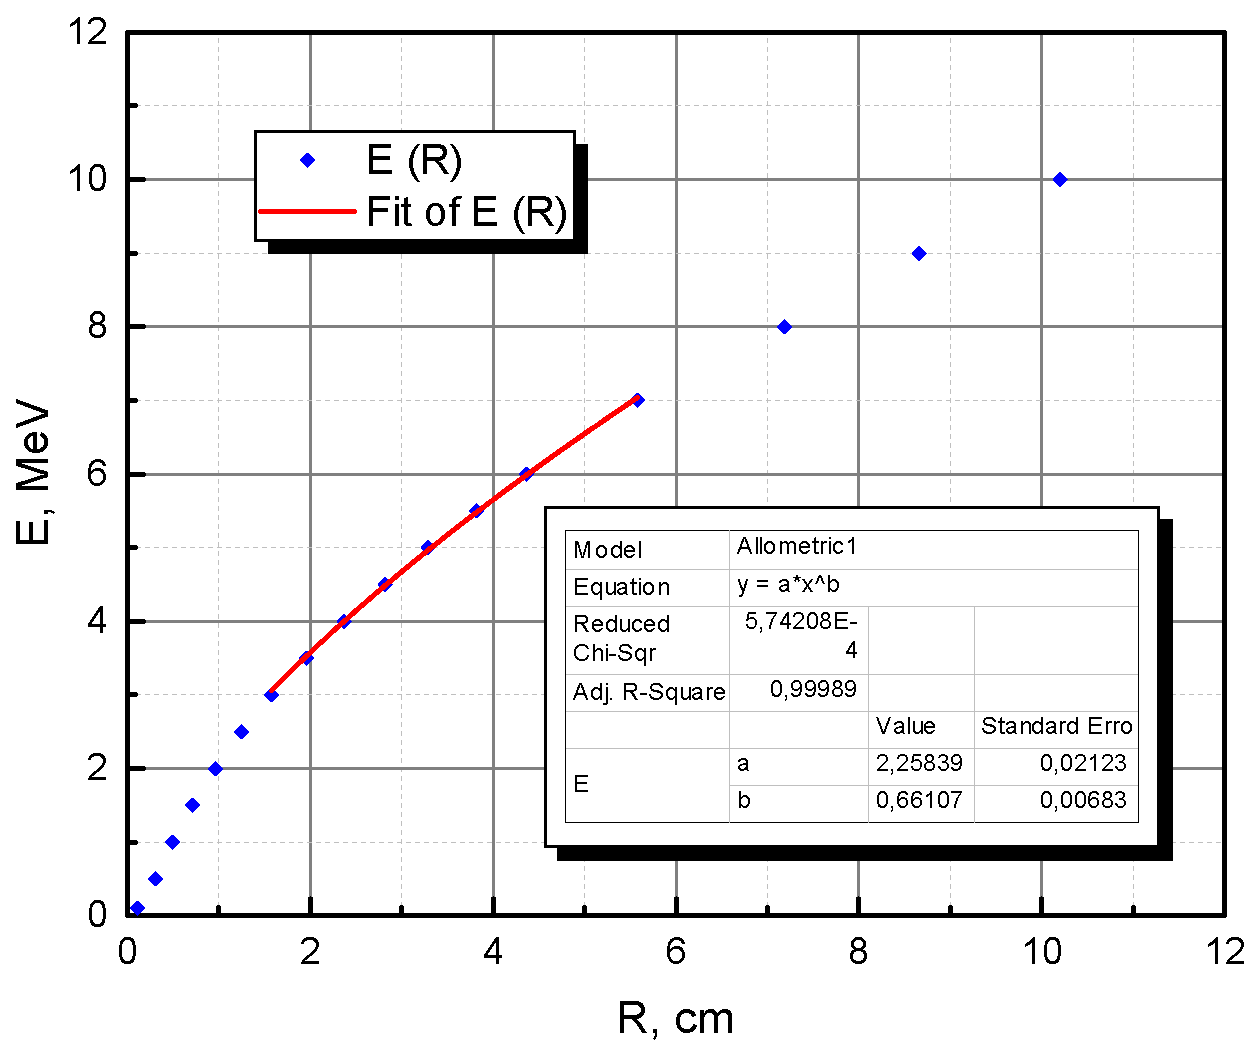
\includegraphics[scale=0.5]{graph4.pdf}}    
		\end{floatrow}
	\end{figure}

\end{document}